\lecture{3}{24. March 2026t}{Feedback Control System Characteristics}

\section{Feedback Control System Characteristics}

\subsection{Basic Concepts and Structure}
Whereas an open-loop control system operates without feedback (see \Cref{fig:oploop3}, a closed-loop system (\Cref{fig:closloop3}) uses a measurement of the outout signal and a comparison with the desired output to generate an error signal that is used by the controller to adjust the actuator, which has certain robustness against disturbances and parameter changes. 

\begin{figure} [ht]
  \centering
  \begin{subfigure}[t]{0.28\textwidth}
    \centering
    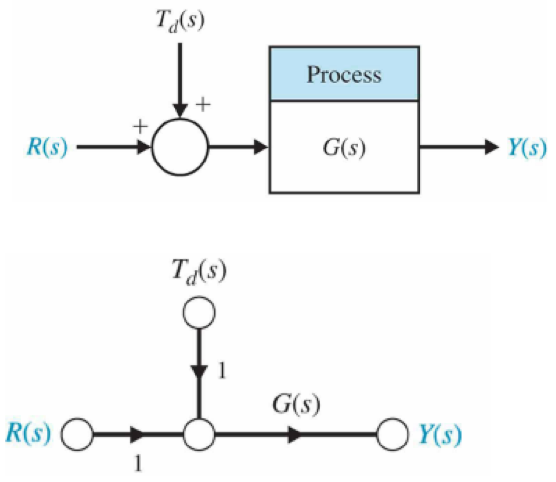
\includegraphics[height=1.25in]{./figures/oploop3.png}
    \caption{Open-loop control system.}
    \label{fig:oploop3}
  \end{subfigure}
  \hfill
  \begin{subfigure}[t]{0.68\textwidth}
    \centering
    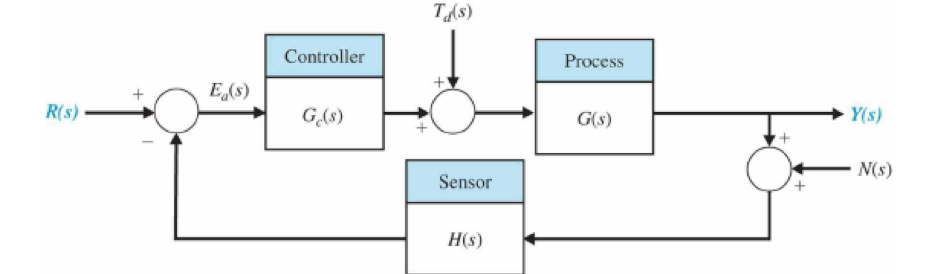
\includegraphics[height=1.25in]{./figures/closloop3.png}
    \caption{Closed-loop control system.}
    \label{fig:closloop3}
  \end{subfigure}
  \caption{Comparison of an open and closed loop control system.}
\end{figure}


\subsection{Error Signal Analysis}
On \Cref{fig:ersigex} we define the tracking error $E(s)$ to be
\begin{equation*}
  E(s) = R(s) - Y(s)
\end{equation*}
because with feedback $H(s) = 1$, the measured output is just the output itself.
I.e. if $Y(S)$ follows $R(s)$ perfectly, then $E(s) = 0$.
On \Cref{fig:ersigex} the system is influenced by three inputs the desired reference $R(s)$, the disturbance $T_d(s)$ and the measurement noise $N(s)$.

\begin{figure} [ht]
  \centering
  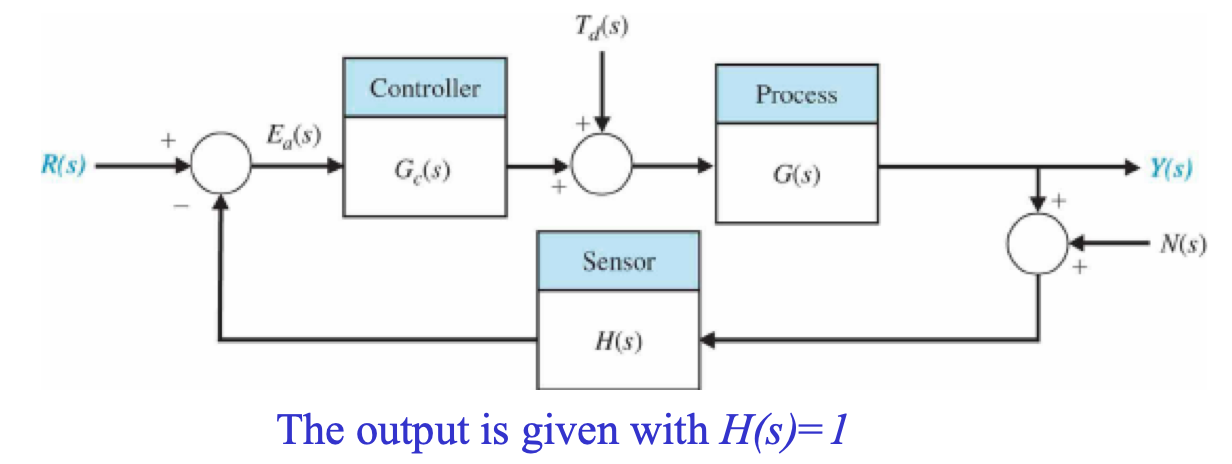
\includegraphics[width=0.5\linewidth]{./figures/ersigex.png}
  \caption{Tracking error with unity feedback, $H(s)=1$.}
  \label{fig:ersigex}
\end{figure}

With feedback $H(s) = 1$, the output $Y(s)$ can be computed as a sum of three contributions.
One from the reference $R(s)$, which is the usual closed-loop transfer function from reference to output:
\begin{equation*}
  Y_R = \frac{G_c G}{1 + G_c G}R
,\end{equation*}
one from the disturbance $T_d(s)$, which shows how much the disturbance affects the output
\begin{equation*}
  Y_T = \frac{G}{1 + G_c G} T_D
,\end{equation*}
and one from the measurement noise
\begin{equation*}
  Y_N = - \frac{G_c G}{1 + G_c G}N
.\end{equation*}
Note the minus sign in the above appears as the noise is in the feedback signal, thus corrupting the measured output and thereby altering the error in the opposite direction.
Which means the output is
\begin{equation*}
  Y(s) = Y_R + Y_T + Y_N = \frac{G_c(s) G(s)}{1 + G_c(s) G(s)}R(s) + \frac{G(s)}{1 + G_c(s) G(s)} T_D(s) - \frac{G_c(s) G(s)}{1 + G_c(s) G(s)}N(s)
.\end{equation*}

The error $E(s)$ is then
\begin{equation*}
  E(s) = R(s) - Y(s) = \frac{1}{1 + G_c(s) G(s)}R(s) - \frac{G(s)}{1 + G_c(s) G(s)}T_d(s) + \frac{G_c (s) G(s)}{1 + G_c(s) G(s)} N(s)
.\end{equation*}

We now define the loop gain $L(s)$ as the total gain you get by going around a feedback loop
\begin{equation*}
  L(s) = G_c(s) G(s) H(s) 
\end{equation*}
and since $H(s) = 1$, 
\begin{equation*}
  L(s) = G_c(s) G(s)
.\end{equation*}
This simplifies the formula for the error to:
\begin{equation*}
  E(s) = \frac{1}{1 + L(s)}R(s) - \frac{G(s)}{1 + L(s)} T_d(s) + \frac{L(s)}{1 + L(s)} N(s)
.\end{equation*}

If we now define the sensitivity function $S(s)$ as
\begin{equation*}
  S(s) = \frac{1}{1 + L(s)}
\end{equation*}
and the complementary sensitivity function $C(s)$ as
\begin{equation*}
  C(s) = \frac{L(s)}{1 + L(s)}
\end{equation*}
then the error becomes
\begin{equation*}
  E(s) = S(s) R(s) - S(s) G(S) T_d(s) + C(s) N(s)
.\end{equation*}
Here, the sensitivity function $S(s) = 1 / (1 + L(s) )$ tells how much of the reference mismatch and disturbance gets through.
From the formula we see that large $L(s)$ leads to small $S(s)$ so large loop gain reduces tracking error $R(s)$ and the effect of disturbance $T_d(s)$
On the other hand, the complementary sensitivity $C(s) = L(s) / (1 + L(s))$ tell how much measurement noise gets through into the error/output.
If $L(s)$ is large, then $C(s) \approx 1$, hence high gain is bad for noise sensitivity. 
Further, we know that
\begin{equation*}
  S(s) + C(s) = 1
\end{equation*}
hence both cannot be small at the same frequency.
Making $S(s)$ small helps tracking and disturbance rejection and making $C(s)$ small helps noise rejection, but improving one tends to worsen the other. 

Generally, disturbances are more important at low frequencies and measurement noise is usually more important at high frequencies.
Therefore, a good controller typically will try to make the loop gain $L(s)$ large at low frequencies and smaller at higher frequencies.
At low frequencies, if $L(s) \gg 1$, then
\begin{equation*}
  S(s) \approx 0, \qquad C(s) \approx 1
\end{equation*}
so the tracking error and disturbance effects are small.
At high frequencies, if $L(s) \ll 1$, then
\begin{equation*}
  S(s) \approx 1, \qquad C(s) \approx 0
\end{equation*}
so measurement noise is suppressed.
I.e. We want the controller to fight slow changes strongly, but ignore very fast noisy fluctuations. 

\subsection{Sensitivity to Parameter Variations}
The input $G(s)$ is time-varying in nature due to uncertainties such as changing environments, aging, and other factors.
These uncertainties will, for open-loop systems result in inaccurate output or low performance, however this can be mitigated in a closed-loop system.
As the process $G(s)$ undergoes a change $\Delta G(s)$ a resulting change in the tracking error $\Delta E(s)$ will occur.
For an open-loop system this will be
\begin{equation*}
  \Delta E(s) = \Delta G(s) G_c(s) R(s)
\end{equation*}
and for a closed loop system it will be:
\begin{align*}
  \Delta E(s) &= \frac{- G_c (s) \Delta G(s)}{\left( 1 + G_c(s) G(s) + G_c(S) \Delta G(s) \right) \left( 1 + G_c (s) G(s) \right)} R(s) \\
              &\approx \frac{- G_c (s) \Delta G(s)}{ \left(  1 + G_c(s) G(s) \right)^2} R(s) \\
    &= \frac{- G_c(s) \Delta G(s)}{\left( 1 + L(s) \right)^2}R(s) \\
    &\approx - \frac{1}{L(s)} \frac{\Delta G(s)}{G(s)} R(s)
.\end{align*}
I.e. for a closed-loop system the error change caused by plant uncertainties is proportional to the relative plant change $\Delta G / G $ divided by the loop gain $L(s)$.
So bigger changes in input result in bigger changes in output but a bigger loop gain results in a smaller error change. 
If e.g. $\left| L(s) \right| = 100$, then the effect of plant variation is suppressed by about a factor 100 at that frequency.

\subsubsection{Sensitivity}
We can define system sensitivity $S$ as
\begin{equation*}
  S = \frac{\Delta T(s) / T(s)}{\Delta G(s) / G(s)}
\end{equation*}
where
\begin{equation*}
  T(s) = \frac{Y(s)}{R(s)}
\end{equation*}
is the closed-loop transfer function from reference to output.
Sensitivity tells how much the transfer function changes, in percentage, when the plant changes by a percentage amount.
So if $S = \num{0,1}$, then a 10\% change in $G$ causes only about a 1\% change in $T$.
This also means that a smaller sensitivity is generally better than a higher one.

For very small changes, percent changes become derivatives:
\begin{equation*}
  S = \frac{\partial T(s) / T(s)}{ \partial G(s) / G(s)} = \frac{\partial \ln T}{\partial \ln G}
\end{equation*}
which is the infinitesimal version of the definition of sensitivity.

We also define $S_G^{T}$ as the sensitivity of $T$ with respect to $G$.
For an open-loop system, then
\begin{equation*}
  T(s) = G_c(s) G(s) \implies S_G^{T} = 1
\end{equation*}
as $T$ is directly proportional to $G$.
Meaning a 1\% change in $G$ results in a 1\% change in the system transfer function $T$, so the loop is fully sensitive.
For a closed-loop with unity feedback
\begin{equation*}
  T(s) = \frac{G_c(s) G(s)}{1 + G_c(s) G(s)} \implies S_G^{T} = \frac{1}{1 + G_c(s) G(s)} = \frac{1}{1 + L(s)}
\end{equation*}
which is exactly the same as the usual sensitivity function.

Instead of asking how much $T$ changes with the whole plant $G$, we can also ask how $T$ changes with some parameter $\alpha$ such as mass, damping, stiffness, time constant, gain constant, etc.
Then:
\begin{equation*}
  S_{\alpha}^{T} = S_G^{T} S_{\alpha}^{G}
\end{equation*}
following the chain-rule.
This can be read as the first parameter, $\alpha$ changes the plant $G$ which then changes the system transfer $T$.
I.e. total sensitivity from $\alpha$ to $T$ is
\begin{equation*}
  (\text{sensitivity of } T \text{ to } G ) \cdot \left( \text{sensitivity of } G \text{ to } \alpha \right)
.\end{equation*}

We can also write
\begin{equation*}
  S_{\alpha}^{T} = \frac{\partial \ln T }{ \partial \ln \alpha}
\end{equation*}
and if
\begin{equation*}
  T(s, \alpha) = \frac{N(s, \alpha)}{D(s, \alpha)}
\end{equation*}
then
\begin{equation*}
  S_{\alpha}^{T} = \frac{\partial \ln N}{\partial \ln \alpha} - \frac{\partial \ln D}{\partial \ln \alpha} = S_{\alpha}^{N} - S_{\alpha}^{T}
.\end{equation*}


\subsection{Disturbance Rejection in Feedback Systems}
A disturbance signal is an unwanted signal that affects the output signal.
From
\begin{equation*}
  E(s) = \frac{1}{1 + L(s)}R(s) - \frac{G(s)}{1 + L(s)}T_d(s) + \frac{L(s)}{1 + L(s)}N(s)
\end{equation*}
with $R(s) = N(s) = 0$ we see the disturbance contribution is
\begin{equation*}
  E_T(s) = - S(s) G(s) T_d(s) = - \frac{G(s)}{1 + L(s)}T_d(s)
\end{equation*}
as mentioned before, large loop gain $L(s) = G_c(s) G(s)$ leads to good disturbance rejection, and disturbance signals are often low frequency so it is desirable to design $G_c(s)$ such that $S(s)$ is small at low frequencies.

To imagine how disturbance arises imagine e.g. a steel bar being moved and rolled by a motor trying to maintain constant speed for the steel bar.
However when the load changes (e.g. due to adding weight to the bar, or drying out of lubricant) the required torque changes too.
That change acts like a disturbance torque $T_d$.
In this scenario, if the controller command is unchanged the rotational speed $\omega$ can drop.

\subsubsection{Open-loop Speed Under Disturbance}
We now want to determine what the speed change of a motor might be due to load disturbance.
For the open-loop motor model on \Cref{fig:disrej}, the error becomes
\begin{equation*}
  E(s) = - \omega(s) = \frac{1}{Js + b + \frac{K_m K_b}{R_a}} T_d(s)
.\end{equation*}
The sign here is negative because a positive load torque opposes motion, so it reduces speed.

If the disturbance is a step torque
\begin{equation*}
  T_d(s) = \frac{D}{s}
\end{equation*}
then by the final value theorem
\begin{equation*}
  \lim_{t \to \infty}E(t) = \lim_{s \to 0}s E(s)
\end{equation*}
which gives
\begin{equation*}
  E(\infty) = \frac{D}{b + \frac{K_m K_b}{R_a}}
\end{equation*}
and since $E = - \omega$
\begin{equation*}
  \omega(\infty) = - \frac{D}{b + \frac{K_m K_b}{R_a}}
.\end{equation*}
This means that a constant extra load torque creates a constant steady speed drop.
I.e. in open-loop, the motor cannot fully reject the step disturbance, it just settles to a lower speed.

\subsubsection{Closed-loop Speed Under Disturbance}
Now, we introduce a feedback controller to reduce the loading disturbance effect as shown on \Cref{fig:disrejfed}.
Here, we also reorganize the system as shown on \Cref{fig:disrejfed}, into
\begin{equation*}
  G_1(s) = \frac{K_a K_m}{R_a}, \qquad G_2(s) = \frac{1}{Js + b}, \qquad H(s) = K_t + \frac{K_b}{K_a}
.\end{equation*}
The disturbance $T_d(s)$ is injected between $G_1$ and $G_2$ and the output is fed back through $H(s)$.

\begin{figure} [ht]
  \centering
  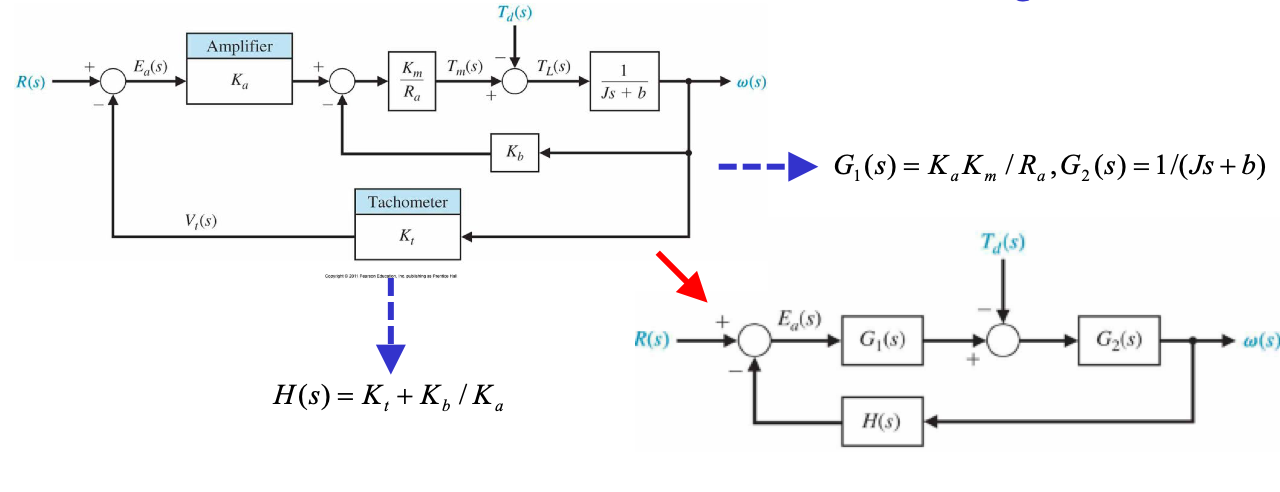
\includegraphics[width=0.8\linewidth]{./figures/disrejfed.png}
  \caption{Closed-loop model.}
  \label{fig:disrejfed}
\end{figure}

For disturbance only, the steady-state error expression for the closed-loop system becomes:
\begin{equation*}
  E(s) = - \omega(s) = \frac{G_2(s)}{1+G_1(s)G_2(s)H(s)}T_d(s)
\end{equation*}
which has the same structure as before:
\begin{equation*}
  \text{disturbance effect} = \frac{\text{plant term}}{1 + \text{loop gain}}
.\end{equation*}

If
\begin{equation*}
  G_1(s) G_2(s) H(S) \gg 1
\end{equation*}
then
\begin{equation*}
  E(s) \approx \frac{1}{G_1(s) H(s)}T_d(s)
\end{equation*}
i.e. for large feedback the disturbance is not much dominated by $G_2$; it is instead suppressed roughly in inverse proportion to the loop gain.
Also
\begin{equation*}
  G_1(s) H(s) = \frac{K_a K_m}{R_a} \left( K_t + \frac{K_b}{K_a} \right)
\end{equation*}
and for $K_a \gg K_b$
\begin{equation*}
  G_1(s) H(s) \approx \frac{K_1 K_m K_t}{R_a}
\end{equation*}
so increasing amplifier gain $K_a$ improves disturbance rejection.

\begin{figure} [ht]
  \centering
  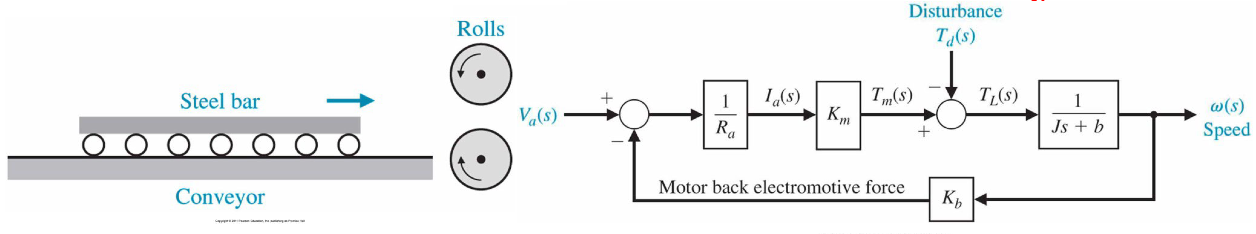
\includegraphics[width=0.8\linewidth]{./figures/disrej.png}
  \caption{Open-loop motor model.}
  \label{fig:disrej}
\end{figure}

With $R(s) = 0$, the closed-loop speed under disturbance becomes
\begin{equation*}
  \omega_{c}(s) = - \frac{1}{Js + b+ \frac{K_m}{R_a} \left( K_t K_a + K_b \right)} T_d(s)
.\end{equation*}
Comparing this with the open-loop version
\begin{equation*}
  \omega_{o}(s) = - \frac{1}{Js + b + \frac{K_{m} K_b}{R_a}} T_d(s)
\end{equation*}
we notice that the closed-loop version has an extra stabilizing term $K_t K_a K_m / R_a$ in the denominator. 

For a step disturbance $T_d(s) = D / s$, the final value theorem gives
\begin{equation*}
  \omega (\infty) = - \frac{D}{b + \frac{K_m}{R_a} \left( K_t K_a + K_b \right)}
\end{equation*}
for sufficiently large $K_a$, this is
\begin{equation*}
  \omega_c(\omega) \approx - \frac{R_a}{K_a K_m K_t} D
.\end{equation*}
Meaning the steady speed drop is now roughly proportional to $1 / K_a$. 

Taking the quotient $\omega_c / \omega_o$ we get
\begin{equation*}
  \frac{\omega_c(\infty)}{\omega_o(\infty)} = \frac{R_a b + K_m K_b}{K_a K_m K_t}
\end{equation*}
which is usually less than \num{0,02}. 
That means the disturbance effect in closed loop systems  can be less than 2\% of what it would be in open loop.

\subsection{Measurement Noise Attenuation}
Measurement noise is noise added in the sensor or measurement path.
The plant output may be fine, but the controller does not see the true output.
Instead it sees
\begin{equation*}
  y_{\text{sensor}} = y + n
\end{equation*}
there $n$ is the noise.
That noise is then fed back, so the controller may react to the noise as if it were a real signal. 
Only looking at the noise contribution to the error we see
\begin{equation*}
  E_n(s) = C(s) N(s) = \frac{L(s)}{1+ L(s)}N(s)
\end{equation*}
where $C(s) = L(s) / (1+L(s))$ is the complementary sensitivity function.
This is complementary to the sensitivity function from above and a trade-off between them is therefore made at a given frequency.

\subsection{The Transient Response Control}
The transient response is the response of a system as a function of time, and must be adjusted until it is satisfactory.
For an open-loop system, the process $G(s)$ must be replaces with a more suitable process, or design the cascade controller $G_c(s)$.
For a closed-loop system, feedback loop parameters can often be adjusted to yield the desired response.

\subsection{Steady-State Error}
The steady state error is the error after the transient response has decayed, leaving only the continuous response.
\begin{equation*}
  e_{ss} = \lim_{t \to \infty}e(t)
.\end{equation*}

In an open loop, the output is just
\begin{equation*}
  Y(s) = G(s) R(s)
\end{equation*}
so the error is
\begin{equation*}
  E_o(s) = R(s) - Y(s) = (1-G(s)) R(s)
\end{equation*}
for a unit step input, $R(s) = 1 / s$, so
\begin{equation*}
  E_o(s) = ( 1 - G(s)) \frac{1}{s}
.\end{equation*}
Now, applying the final value theorem we get:
\begin{equation*}
  e_o(\infty) = \lim_{s \to 0}sE_o(s) = \lim_{s \to 0}s \left( 1 - G(s) \right)\frac{1}{s} = 1 - G(0)
.\end{equation*}
I.e. the steady-state error depends on the DC gain $G(0)$.
If $G(0) = 1$, then $e_o(\infty) = 0$, however $G(0) \neq 1$ leads to a nonzero steady state error.

For a closed loop system, the feedback means a much smaller error is produced.
For unity feedback $H(s) = 1$, the error transfer function is
\begin{equation*}
  E_c(s) = \frac{1}{1 + G_c(s) G(s)}R(S)
.\end{equation*}
For a unit step input
\begin{equation*}
  E_c(s) = \frac{1}{1 + G_c(s) G(s)}\frac{1}{s}
.\end{equation*}
Now, applying the final value theorem, we get
\begin{equation*}
  e_c(\infty) = \lim_{s \to 0}s E_c(s) = \lim_{s \to 0}s \left( \frac{1}{1  + G_c(s) G(s)} \frac{1}{s} \right)
\end{equation*}
so
\begin{equation*}
  e_c(\infty) = \frac{1}{1 + G_c(0) G(0)}
\end{equation*}
or using the DC loop gain:
\begin{equation*}
  e_c(\infty) = \frac{1}{1 + L(0)}
.\end{equation*}
So if the DC loop gain is large, then the steady-state error is small.


\subsection{The Cost of Feedback}
In general, feedback is very useful to make more accurate systems, however one must always keep the cost of adding said feedback in mind before deciding if it is worth the investment.
Adding feedback leads to increased complexity, as sensors, which are expensive, noisy, and inaccurate, need to be added.
The closed loop gain of a feedback system will also decrease by a factor of $1 / (1 + G_c(s) G(s))$.
Further, feedback introduces possible instability of the system, which does not arise for open-loop systems.
